\section{Resultados e discussões}
\subsection{Sistema massa-mola}
%Done: freq de oscilações
%Done: const elástica da mola
%Done: relação massa ~ freq
A partir dos dados extraídos do Tracker, resumidos nas \cref{molaG,molaP,molaG2m}, é notável observar o comportamento senoidal de todos os sistemas. É possível estimar a frequência do sistema massa-mola pela observação gráfica. Em \cref{molaG} a observação indica aproximadamente 1 oscilação por segundo. Enquanto em \cref{molaP} obtêm-se pouco mais de uma oscilação por segundo. E, em \cref{molaG2m} pouco menos de 1 oscilação por segundo.

\begin{figure}[h]
    \centering
    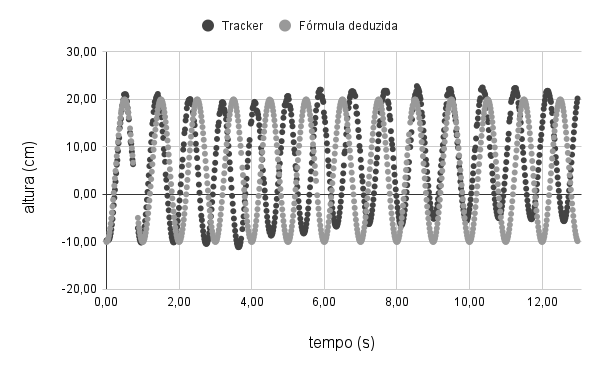
\includegraphics[width=.5\linewidth]{fig/molaG}
    \caption{Para mola grande com massa de \qty{100}{g}, gráfico de dispersão dos dados obtidos no Tracker em comparação aos valores nos mesmos instantes de tempo com a função horária deduzida}\label{molaG}
\end{figure}

\begin{figure}[h]
    \centering
    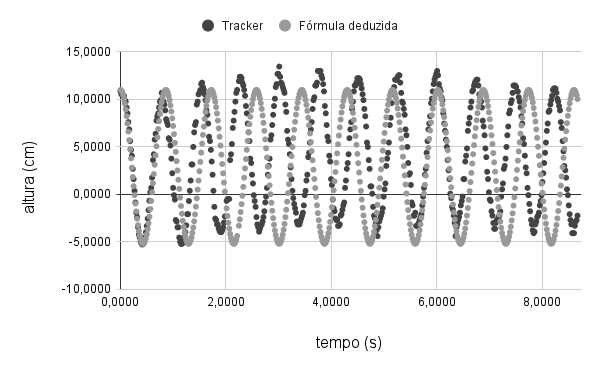
\includegraphics[width=.5\linewidth]{fig/molaP}
    \caption{Para mola pequena com massa de \qty{100}{g}, gráfico de dispersão dos dados obtidos no Tracker em comparação aos valores nos mesmos instantes de tempo com a função horária deduzida}\label{molaP}
\end{figure}
 
No entanto, podemos também nos aproveitar do comportamento dos sistemas e obter uma equação para descrever cada um dos sistemas a partir da função horária da posição da massa considerando que tenha comportamento de um oscilador harmônico simples: 

\begin{align*}
    x(t) = A\cos(\omega t + \psi) + x_0
\end{align*}

Para o sistema com a mola maior e a massa de \qty{100}{\gram}, considerando os primeiros períodos, obtemos que os pontos de máximo e mínimo são: \(x(0) = \qty{-10}{cm}\), \(x(0,50) = \qty{20}{cm}\). Então, podemos extrair a função horária:

\begin{align*}
    x_{Gm}(t) = A\cos(\omega t + \psi) + x_{Gm0}\\
    x_{Gm}(0) = A + x_{Gm0} = \qty{20}{cm} \\
    x_{Gm}(1) = -A + x_{Gm0} = \qty{-10}{cm} \\
    \implies x_{Gm0} = \qty{5}{cm}\\
    \implies A = \qty{20}{cm} - \qty{5}{cm} = \qty{15}{cm}\\
    \text{Além de que:}\\
    x_{Gm}(0) \text{é mínimo} \implies \cos(\psi) = -1\\
    \implies \psi = \pi\\
    x_{Gm}(0,50) \text{é máximo} \implies \cos(0,5\omega + \pi) = 1\\
    \implies \omega = 2 \pi\\
    \implies x_{Gm}(t) = 15\cos(2\pi t + \pi) + 5\\
    \implies x_{Gm}(t) = -15\cos(2\pi t) + 5
\end{align*}

Esta é a fórmula deduzida para o sistema massa-mola apresentada em cinza na \cref{molaG}. É notável que a fórmula descreve bem o sistema nos períodos iniciais e começa a se comportar de maneira diferente ao longo de mais períodos. Esta divergência decorre de: (1) a dispersão de energia na forma de calor no sistema real, (2) a trepidação do sistema no eixo x, não oscilando perfeitamente na vertical, (3) a trepidação da câmera que registra o sistema, causando diferenças na altura absoluta da massa com relação a altura observada no software Tracker.

O mesmo processo pode ser utilizada para extrair a função horária da mola menor:

\begin{align*}
x_{pm}(t) = 8,1 \cos(\frac{\pi}{0,43}t) + 2,9
\end{align*}

    Que também apresenta divergências com relação aos dados extraídos do Tracker pela mesma justificativa que a mola maior, conforme observável na \cref{molaP}.
    Com as funções horárias é possível determinar a frequência dos osciladores:

\begin{align*}
    \nu = \frac{\omega}{2\pi}\\
    \nu_{pm} = \frac{\pi}{\num{0,43} \cdot 2\pi} = \num{1,16}\\ 
    \nu_{Gm} = \frac{2\pi}{2\pi} = 1
\end{align*}

Em que, \(\nu_{pm}\) é a frequência da mola pequena com massa de \qty{100}{g} e \(\nu_{Gm}\) é a mola grande com massa de \qty{100}{g}. Obtemos então, resultados compatíveis com a análise gráfica.

É possível determinar também a constante elástica das molas:
\begin{align*}
   k = \omega^2 \cdot m\\
   k_{pm} = {(\pi\qty{2}{\per\second})}^2 \cdot \qty{0.1}{\kilo\gram}\\
   k_{pm} = \qty{3,95}{\N\per\meter}\\
   k_{Gm} = {(\frac{\pi}{0.43}\qty{1}{\per\second})}^2 \cdot \qty{0.1}{\kg}\\
   k_{Gm} = \qty{5.34}{\N\per\meter} 
\end{align*}

A frequência de oscilação do sistema é determinada por \(\frac{\omega}{2 \pi}  = \nu\), com \(\omega^2 = \frac{k}{m}\), portanto, a frequência deve ser inversamente proporcional à raiz quadrada da massa. Podemos averiguar isso observando a frequência para o sistema com a massa grande com \qty{200}{\g}. A função derivada para esta mola é \(x_{G2m} = 8.84\cos(\frac{\pi}{0.66}t) -11.16\), é possível observar a comparação entre esta função e os dados extraídos do Tracker na \cref{molaG2m}. Desta função, podemos extrair \(\nu = \cfrac{\pi}{0.66 \cdot 2 \cdot \pi} = \qty{0.76}{\per\second}\). Como esperado, o valor obtido é menor que a frequência para a mesma mola com uma massa menor.   

\begin{figure}[h]
    \centering
    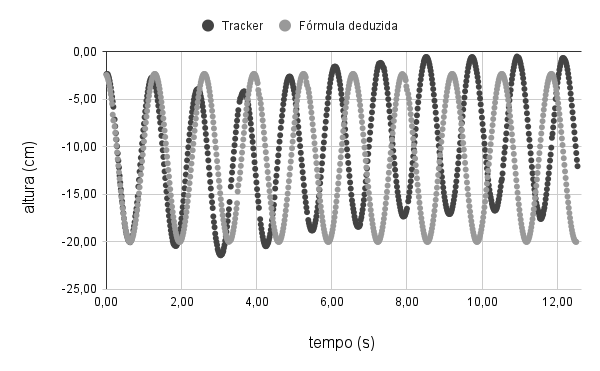
\includegraphics[width=.5\linewidth]{fig/molaG2m}
    \caption{Para mola grande com peso de \qty{200}{\g}, a figura apresenta os dados extraídos do software Tracker em comparação com os valores obtidos nos mesmos instantes de tempo para uma função horária deduzida para este oscilador}
    \label{molaG2m}
\end{figure}

\subsection{Pêndulo de Wilberforce}
Neste experimento, foi analisado o comportamento do Pêndulo de Wilberforce, um sistema que exemplifica de forma clara o fenômeno de oscilações acopladas. O aspecto mais notável do pêndulo é a transferência gradual de energia entre os modos de oscilação longitudinal e rotacional, resultando em alternâncias periódicas entre esses movimentos.

A origem dessa transferência de energia está no acoplamento entre os dois modos de oscilação, causado pelas propriedades geométricas e elásticas da mola. Quando a massa oscila verticalmente, a mola se comprime e se estende. Devido à sua estrutura helicoidal, essas variações induzem uma torção no sistema, influenciando o movimento rotacional. Esse acoplamento permite que a energia seja transferida entre os modos de oscilação, caracterizando o sistema como um oscilador acoplado .

Para que a transferência de energia entre os modos longitudinal e rotacional seja eficiente, é fundamental que suas frequências naturais sejam próximas. Uma forma de ajustar essa proximidade é modificando a frequência do modo rotacional por meio da posição dos discos laterais, o que altera o momento de inércia da massa suspensa. Quando essa condição é atingida, o sistema pode entrar em ressonância, o que favorece a troca contínua de energia entre os dois modos de oscilação.

Durante esse processo, a energia potencial elástica associada à compressão e extensão da mola (modo longitudinal) e a energia potencial de torção (modo rotacional) são convertidas em suas respectivas formas de energia cinética. A energia cinética translacional está relacionada ao movimento vertical da massa, enquanto a energia cinética rotacional está associada à sua rotação. A alternância entre esses modos resulta em uma oscilação da amplitude de cada movimento, evidenciando a transferência gradual de energia no sistema.

Esse comportamento do Pêndulo de Wilberforce não apenas ilustra princípios fundamentais da física de oscilações acopladas, mas também encontra analogias em sistemas do cotidiano, como a maquina de lavar. Uma vez que, como um pêndulo de Wilberforce, ela realiza oscilações no 
eixo rotacional e oscilações no eixo longitudinal. Essa dinâmica de um oscilador acoplado, lhe confere a propriedade de transferência 
gradual de energia entre os modos de oscilação, e dependência da ressonância entre as oscilações para melhor funcionamento do equipamento.
Dessa forma, se a frequência da rotação estiver muito descalibrada, devido ao acumulo de massa em um ponto do cesto da máquina por exemplo,
pode ocasionar em um transferência excessiva de energia para a oscilação longitudinal, o que pode danificar o máquina.

\subsection{Pêndulo de Torção}  

Para analisar o comportamento do pêndulo de torção em diferentes meios, foi medido o tempo necessário para realizar oscilações tanto no 
ar quanto no óleo. Dessas medições, pontuou-se as 5 primeiras oscilações, e ao realizar uma regressão linear, obteve-se uma expressão que corresponde
ao comportamento do pêndulo, tanto no ar quanto no óleo, como é possível observar nas imagens \label{Troçãonoar} e \label{Torçãonoóleo}.
Dessa forma, utilizando as expressões que correspondem ao comportamento do pêndulo em diferentes meios para calcular qual seria o tempo necessário
para se realizar 10 oscilações, temos:

\begin{figure}[H]
	\centering
	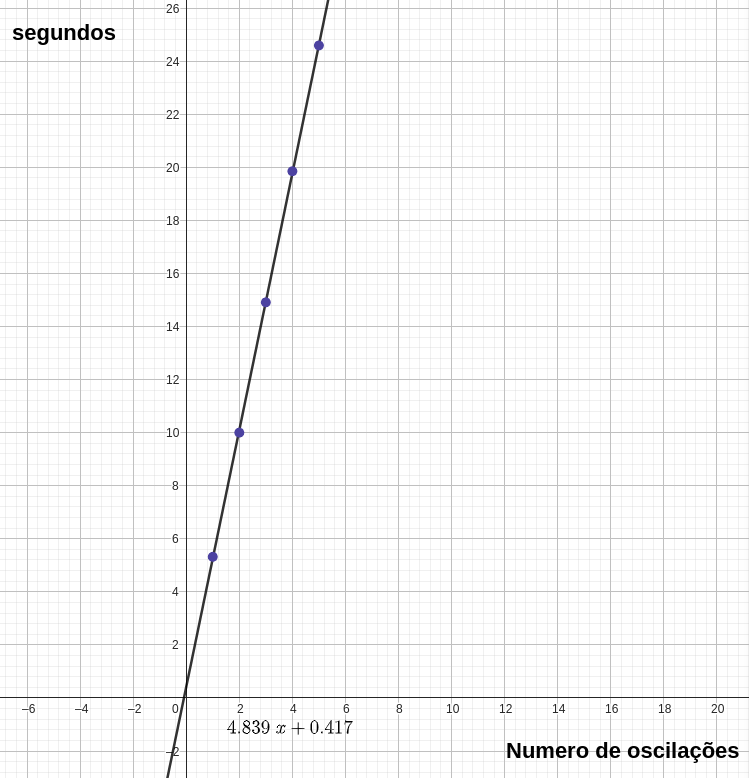
\includegraphics[width=0.35\linewidth]{fig/Torção no ar.png}
	\caption{Gráfico do numero de oscilações do pêndulo de torção no ar por tempo, tendo feita a regressão linear com 5 pontos}
	\label{Torçãonoar}
\end{figure}

\begin{figure}[H]
	\centering
	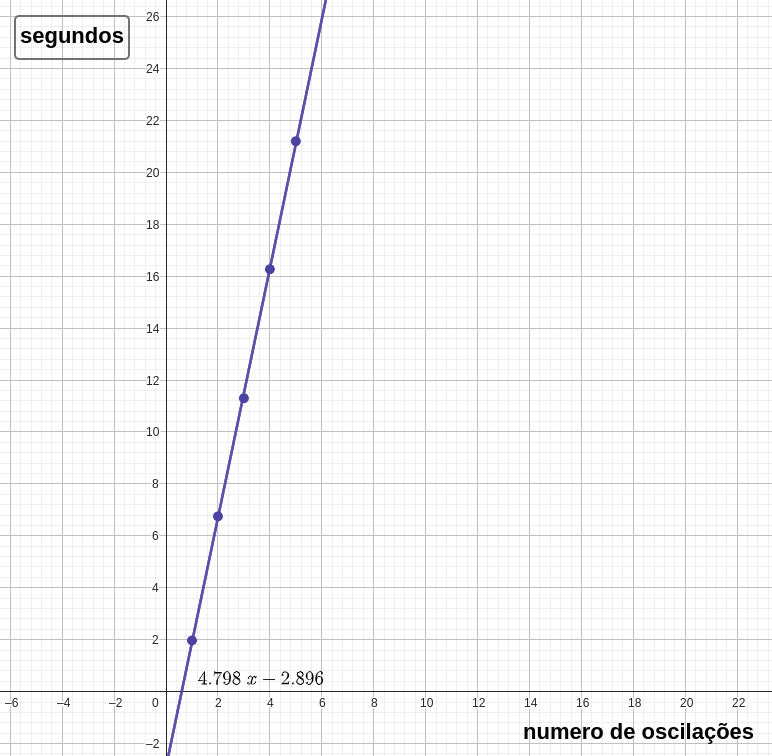
\includegraphics[width=0.35\linewidth]{fig/Oscilações no óleo.png}
	\caption{Gráfico do numero de oscilações do pêndulo de torção no óleo por tempo, tendo feita a regressão linear com 5 pontos}
	\label{Torçãonoóleo}
\end{figure}

Pêndulo no ar:
\begin{align*}
	f(x) &= 4,839x +  0,417 \text{ Sendo "f(x)" o tempo em segundos, e "x" o numero de oscilações} \\
 	f(x) &= 4,839 * 10 + 0,417\\
    f(x) &= \qty{48,807}{s}	
\end{align*}

Pêndulo no óleo:
\begin{align*}
	f(x) &= 4,798x -  2,896 \text{ Sendo "f(x)" o tempo em segundos, e "x" o numero de oscilações}\\
	f(x) &= 4,798 * 10 - 2,896\\
	f(x) &= \qty{45,084}{s}
\end{align*}

\begin{table}[H]
	\caption{Dados obtidos empiricamente do pêndulo de Torção no ar} \label{tabelaar}
	\begin{center}
		\begin{tabular}{c c c}
			\hline
			Oscilação & Tempo (s) & Variação do Tempo (s) \\
			\hline
			1 & 00:05.32 & 00:05.32\\
			2 & 00:10.00 & 00:04.68\\
			3 & 00:14.91 & 00:04.91\\
			4 & 00:19.85 & 00:04.94\\
			5 & 00:24.59 & 00:04.74\\
			6 & 00:29.50 & 00:04.91\\
			7 & 00:34.32 & 00:04.82\\
			8 & 00:39.24 & 00:04.92\\
			9 & 00:44.23 & 00:04.99\\
			10 & 00:48.94 & 00:04.71\\
			\hline
		\end{tabular}
	\end{center}
\end{table}

\begin{table}[H]
	\caption{Dados obtidos empiricamente do pêndulo de Torção no óleo} \label{tabelaóleo}
	\begin{center}
		\begin{tabular}{c c c}
			\hline
			Oscilação & Tempo (s) & Variação do Tempo (s) \\
			\hline
			1 & 00:01.97 & 00:01.97\\
			2 & 00:06.75 & 00:04.78\\
			3 & 00:11.30 & 00:04.55\\
			4 & 00:16.27 & 00:04.97\\
			5 & 00:21.20 & 00:04.93\\
			6 & 00:26.14 & 00:04.94\\
			7 & 00:31.08 & 00:04.94\\
			8 & 00:35.83 & 00:04.75\\
			9 & 00:40.42 & 00:04.59\\
			10 & 00:45.46 & 00:05.04\\
			\hline
		\end{tabular}
	\end{center}
\end{table}

Como observado nas tabelas \ref{tabelaar} e \ref{tabelaóleo}, as previsões da regressão linear estão de acordo com os valores empíricos. Além disso, a análise dos dados permite concluir que, no ar, o pêndulo apresentou oscilações com variações de tempo bastante regulares, com valor médio aproximado de \qty{4,86}{s} por oscilação. Isso sugere que, nesse meio de baixa resistência, o movimento mantém sua periodicidade e conserva energia por mais tempo.

Já no óleo, embora a média das oscilações também tenha se mantido próxima a \qty{4,85}{s}, a primeira oscilação foi significativamente mais curta (\qty{1,97}{s}), o que pode indicar um erro experimental ou falha na cronometragem. Ao desconsiderar essa medida inicial, a média passa para \qty{4,83}{s}, valor mais coerente com o esperado para um sistema amortecido.

Assim, ao excluir a primeira medição, conclui-se que o pêndulo no ar representa um sistema quase conservativo, enquanto o pêndulo no óleo evidencia a ação de um meio viscoso, que dissipa energia com mais intensidade, reduzindo a amplitude das oscilações com o tempo.

\subsection{Ondas}
%TODO: como o ocorre formação de nós;
%TODO: qual a diff entre esfera que vibra e e as molas?
A formação de ondas transversais na mola maior resultou em ondas se propagando ao longo da mola formando picos e vales na mola transversais ao deslocamento da onda. Ao agitar suficientemente e consistentemente rápido tornou-se possível notar que uma quantidade fixa de vales e picos se formaram em pontos fixos da mola com alguns. Nos pontos de encontro entre um vale e um pico a posição do segmento de mola permaneceu constante, isto é o que denomina-se um nó. Este comportamento é explicado pela reflexão das ondas que ao chegarem do lado oposto ao que foram formadas invertem de fase, então, se a frequência é tal que caiba um número inteiro de meio comprimentos de ondas na mola, as fases opostas se cancelam formando nós e as fases iguais se somam, formando vales e picos mais evidentes. 

Ao criar ondas longitudinais ao longo da mola menor, não foi possível observar a formação de nós. Provavelmente devido à não executar os impulsos com a frequência correta para o cenário anteriormente descrito aconteça. 
    
Por fim, as esferas presas às pontas das cordas vibram à uma frequência fixa. Portanto, a única forma de observar a formação de nós é segurando a corda com comprimento suficiente para que, dada a frequência da esfera, o número correto de ondas seja formado. Exatamente este fenômeno foi observado, ainda, é possível notar que ao aumentar suficientemente o comprimento é possível notar a formação de mais nós apenas quando o comprimento foi exato. Ademais, entre a formação de \(n\) nós e \(n+1\) nós, os nós formados anteriormente ``desaparecem'' até que o comprimento seja suficiente para formação dos nós seguintes.



